\PassOptionsToPackage{usenames,dvipsnames}{xcolor}
\documentclass[usenames, dvipsnames]{beamer}
\usepackage[utf8]{inputenc}
\usepackage[brazil]{babel}
\usepackage{graphicx}
\usepackage{multimedia}
\usepackage{smartdiagram}
\usepackage{xcolor}
\usepackage{tikz}
\usetikzlibrary{shapes,arrows}
\usepackage{braket}
\usepackage{dsfont}
\usepackage{amsmath,amssymb}
\usepackage{empheq}
\usepackage[most]{tcolorbox}
\usepackage{subfig}
\usepackage{verbatim}
\usepackage{hyperref}

% For greek words:
\usepackage[LGR,T1]{fontenc}
\newcommand{\textgreek}[1]{\begingroup\fontencoding{LGR}\selectfont#1\endgroup}
% ###########################


\newtcbox{\mymath}[1][]{%
    nobeforeafter, math upper, tcbox raise base,
    enhanced, colframe=blue!50!green!50,
    colback=blue!10!white, boxrule=1pt,
    #1}
\newtcbox{\mymathred}[1][]{%
    nobeforeafter, math upper, tcbox raise base,
    enhanced, colframe=red!50!black!50,
    colback=red!10!white, boxrule=1pt,
    #1}

%\usetheme{Bergen}
%\usetheme{Berkeley}
%\usetheme{Copenhagen}
\usetheme{CambridgeUS}
%\usetheme{Szeged}
% \usetheme{Goettingen}
% \usetheme{bjeldbak/beamerthemebjeldbak}
%\usecolortheme{seahorse}
% \usecolortheme{beaver}

% O bloco de comandos a seguir garante que a cada início de seção
% surge o sumário com a seção corrente em destaque
%
%\AtBeginSection[]
%{
%  \begin{frame}
%    \frametitle{Sumário}
%    \tableofcontents[currentsection]
%  \end{frame}
%}


\title[introduction to topological insulators] %optional
{Topological Insulators}
\subtitle{a short introduction}

\author{\textbf {Marcos H. Lima de Medeiros}}
\institute[IFUSP] % (optional)
{
  Instituto de Física\\
  Universidade de São Paulo
}
\date[VLC 2013] % (optional)
{October, 2018}
%\logo{\includegraphics[height=0.6cm]{usp.png}}



% \graphicspath{{phases_of_matter/}}


\begin{document}
\frame{\titlepage}

\begin{frame}
 \frametitle{Summary}
 \tableofcontents[pausesections]
\end{frame}


%%%%%%%%%%%%%%%%%%%%%%%%%%%%%%%%%%%%%%%%%%%%%%%%%%%%%
      %%%%%%%%%%%%% Phases of Matter %%%%%%%%%%%%
%%%%%%%%%%%%%%%%%%%%%%%%%%%%%%%%%%%%%%%%%%%%%%%%%%%%%

\begin{frame}
    \frametitle{2016 Nobel prize}
    \includegraphics[width=1\textwidth]{phases_of_matter/nobel_phys_2016.jpg}
\end{frame}


\section{Phases of Matter}

\begin{frame}
    \frametitle{States (phases) of Matter}

    \begin{block}{}
        Classically, when we change temperature we may have
        phase transitions
    \end{block}

    \begin{columns}
    \column{0.3\textwidth}
        \begin{itemize}
            \item Solid
            \item Liquid
            \item Gas
            \item Plasma
        \end{itemize}

    \column{0.70\textwidth}
        \includegraphics[width=1\textwidth]{phases_of_matter/tirinha_states_matter.jpg}
    \end{columns}

\end{frame}

\begin{frame}

    \frametitle{Symmetry and order}
    \begin{block}{Landau paradigm}
        Phase transitions are related to (local) order parameters:
        more symmetric less oredered the system
    \end{block}

    \begin{columns}
    \column{0.5\textwidth}
    \begin{itemize}
        \item Solid
        \item Liquid
        \item Gas
        \item Plasma
    \end{itemize}
    \column{0.5\textwidth}
        \includegraphics[width=0.5\textwidth]{phases_of_matter/setas_order_symmetry.png}
    \end{columns}

\end{frame}

\begin{frame}

    \frametitle{Symmetry and order}
    \begin{block}{Landau paradigm}
        Phase transitions are related to (local) order parameters:
        more symmetric less oredered the system
    \end{block}

    \begin{columns}
    \column{0.5\textwidth}
    \begin{itemize}
        \item Ferromagnetic
        \item Antiferromagnetic
        \item Paramagnetic
    \end{itemize}
    \column{0.5\textwidth}
        \includegraphics[width=0.5\textwidth]{phases_of_matter/spin_chains.png}
    \end{columns}

\end{frame}


%%%%%%%%%%%%%%%%%%%%%%%%%%%%%%%%%%%%%%%%%%%%%%%%%%%%%
      %%%%%%%  Quantum Phases of Matter %%%%%%%
%%%%%%%%%%%%%%%%%%%%%%%%%%%%%%%%%%%%%%%%%%%%%%%%%%%%%


%%%%%%%%%%%%%%%%%%%%%%%%%%%%%%%%%%%%%%%%%%%%%%%%%%%%%
      %%%%% Topological  Phases of Matter %%%%
%%%%%%%%%%%%%%%%%%%%%%%%%%%%%%%%%%%%%%%%%%%%%%%%%%%%%
\section{Topology in matter}


\begin{frame}
    \frametitle{In little bit of Topology}

    Topology $=$ (\textgreek{t'opos}) $+$ (\textgreek{l'ogos})
    $=$ place $+$ study


    \begin{columns}
    \column{0.5\textwidth}
        \begin{block}{Gauss-Bonnet formula:}
            \begin{equation}
                \int_S \kappa_1 \kappa_2 dA = 2\pi\chi = 2\pi(2-g)
            \end{equation}
                esphere : $2\pi (2-0) = 4\pi$

                torus : $2\pi (2-1) = 2\pi$
        \end{block}
    \column{0.5\textwidth}
        \includegraphics[width=.9\textwidth]{phases_of_matter/topological_transitions_geometry.png}
    \end{columns}

\end{frame}

\begin{frame}
    \frametitle{Trivial Insulators}
    \begin{columns}

        \column{0.5\textwidth}
            Band theory of solids: insulators has a gapped band structure

            \only<1>{\includegraphics[width=.7\textwidth]{phases_of_matter/bands_insulator.png}}
            \only<2->{\includegraphics[width=.7\textwidth]{phases_of_matter/bands_electron_hole.png}}

        \column{0.5\textwidth}
            \only<3->{\begin{block}{The Dirac sea}
                The vacuum is also "gapped".
                \includegraphics[width=.7\textwidth]{phases_of_matter/dirac_sea.png}
            \end{block}}

    \end{columns}

\end{frame}



\begin{frame}
    \frametitle{Quantum Hall Effect}
    \begin{columns}
        \column{0.5\textwidth}
        \begin{block}{}
            \begin{equation}
                H(\alpha) = (1-\alpha)H + \alpha H^{\prime} \nonumber
            \end{equation}
        \end{block}
        \begin{center}
            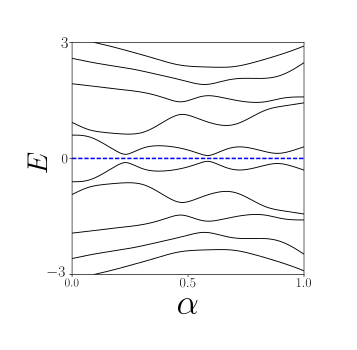
\includegraphics[width=.7\textwidth]{phases_of_matter/equivalent_gapped_hamiltonians.png}
        \end{center}

        \column{0.4\textwidth}
        \pause
        Is every gapped system topological equivalent to the vaccum?
        \pause

        Answer: No!
        \begin{block}{}
            \includegraphics[width=\textwidth]{phases_of_matter/non_equivalent_systems.png}
        \end{block}
    \end{columns}

\end{frame}


\begin{frame}
    \frametitle{First topological insulator}

    \begin{columns}

    \column{0.5\textwidth}
        Landau levels:
        \begin{equation}
            E = \hbar \omega_c \left( m +  \frac{1}{2}\right) \nonumber
        \end{equation}

        Hall conductivity:
        \begin{equation}
            \sigma_{xy} = \frac{Ne^2}{2\pi\hbar} \nonumber
        \end{equation}


    \column{0.5\textwidth}
    Berry phase associated to Bloch wavefunctions:

    \begin{equation}
        \mathcal{F}^m(\mathbf{k}) = i \nabla \times \Braket{u_m(k)|\nabla_k|u_m(k)} \nonumber
    \end{equation}

    \begin{block}{Thouless, Kohmoto, Nightingale and den Nijs(TKNN)}
        \[N =  \sum_{m=1}^{M} \int \frac{d^2\mathbf{k}}{2\pi}  \mathcal{F}^m_{k_xk_y} \]
    \end{block}

    \end{columns}

\end{frame}




%%%%%%%%%%%%%%%%%%%%%%%%%%%%%%%%%%%%%%%%%%%%%%%%%%%%%
      %%%%%%%%%%  Why does it matters %%%%%%%%
%%%%%%%%%%%%%%%%%%%%%%%%%%%%%%%%%%%%%%%%%%%%%%%%%%%%%
\section{Topological Insulators}

\begin{frame}
    \frametitle{2D Tolopological Insulators}

        Also known as Quantum spin Hall system.

        \includegraphics[width=\textwidth]{phases_of_matter/different_hall_effects.jpg}

\end{frame}

\begin{frame}
    \frametitle{Transport in Tolopological Insulators}

    \begin{columns}

    \column{0.5\textwidth}
        'Hidden' edge-states only for spin (?):

        \includegraphics[width=\textwidth]{phases_of_matter/110_delta_0_E_426.png}

    \column{0.5\textwidth}
        Tunable 2D topological insulator.

        \includegraphics[width=\textwidth]{phases_of_matter/3_plots_juntos.png}
    \end{columns}

\end{frame}

\begin{frame}
      \centering \Huge
      \textbf{\emph{Thank you}}
\end{frame}


\end{document}
